\documentclass[11pt, report, french]{scrreprt}

\usepackage{hyperref}

\usepackage{float}


%encoding
%--------------------------------------
\usepackage[utf8]{inputenc}
\usepackage[T1]{fontenc}
%--------------------------------------

%French-specific commands
%--------------------------------------
\usepackage{babel}
\usepackage[autolanguage]{numprint}
%--------------------------------------

%Hyphenation rules
%--------------------------------------
\usepackage{hyphenat}
\hyphenation{mathéma-tiques récu-pérer}
%--------------------------------------

%Maths box
%--------------------------------------
\usepackage{amsmath}
\usepackage[most]{tcolorbox}

\tcbset{colback=yellow!10!white, colframe=red!50!black, 
	highlight math style= {enhanced, %<-- needed for the ’remember’ options
		colframe=red,colback=red!10!white,boxsep=0pt}
}
%--------------------------------------

%code blocs
%--------------------------------------

\usepackage{listings}
\usepackage{xcolor}

\definecolor{codegreen}{rgb}{0,0.6,0}
\definecolor{codegray}{rgb}{0.5,0.5,0.5}
\definecolor{codepurple}{rgb}{0.58,0,0.82}
\definecolor{backcolour}{rgb}{0.95,0.95,0.92}

\lstdefinestyle{mystyle}{
	backgroundcolor=\color{backcolour},   
	commentstyle=\color{codegreen},
	keywordstyle=\color{magenta},
	numberstyle=\tiny\color{codegray},
	stringstyle=\color{codepurple},
	basicstyle=\ttfamily\footnotesize,
	breakatwhitespace=false,         
	breaklines=true,                 
	captionpos=b,                    
	keepspaces=true,                 
	numbers=left,                    
	numbersep=5pt,                  
	showspaces=false,                
	showstringspaces=false,
	showtabs=false,                  
	tabsize=2
}

\lstset{style=mystyle}
%--------------------------------------

\usepackage[margin=2cm]{geometry}
\usepackage{graphicx}

\title{
	\includegraphics[scale=1]{img/logo.png}\\[4cm]
	\huge\textbf{Identification des titres musicaux}
}
\subtitle{Méthode de fingerprinting\\[2cm]}
\author{
	Othman EL HOUFI \\ Mohamed DIAWARA \\[2cm]
	\textbf{M1 Systèmes Intelligents et Communicants} \\[2cm]
	
	Rapporteur : Dan VODISLAV \\
	Tuteur technique : Dimitris KOTZINOS \\
	Encadrant de gestion de projet : Tianxiao LIU \\[2.5cm]
}

\date{\today}

\begin{document}
	
	%%%%%TITLE%%%%%
	\begin{titlepage}
		\maketitle
	\end{titlepage}

\chapter*{Remerciement}
C’est avec un grand plaisir que nous réservons cette page en signe de gratitude et de profonde reconnaissance à tous ceux qui ont bien voulu apporter l’assistance nécessaire au bon déroulement de ce travail.\\

Nos remerciements les plus sincères vont à M. Dimitris Kotzinos, notre tuteur technique et enseignant à l'Université de Cergy Pontoise pour son soutien et ses recommandations  judicieuses.\\

Nous remercions M. LIU Tianxiao, notre encadrant à l’Université de Cergy pour sa confiance, ses conseils, son accompagnement, son encouragement ainsi que pour la qualité et la complémentarité de son encadrement. Il nous a ouvert son savoir-faire et ses expériences pour un insigne accroissement de connaissances acquises. \\

M. LIU nous nous sommes très honorés de travailler avec vous et nous tenons à vous adresser nos remerciements les plus  profondes.  Nous adressons nos sincères remerciements à tous les membres du jury qui nous ont fait l’honneur d’accepter de prendre part à ce jury et surtout de lire et d’expertiser notre travail. Et nous souhaitons également remercier tout le corps professoral du département Informatique de l'Université de Cergy pour la qualité de l’enseignement. \\\par
En somme, pour tous ceux qui n’ont pas hésité à nous accorder leur soutien, leur amitié ou leur expérience tout au long de nos années d’études et qui ont accompagné nos pas d’une part ou d’une autre, veuillez accepter nos modestes remerciements.\\

%%%%%TABLE OF CONTENT%%%%%
\tableofcontents

\chapter{Introduction}
\section{Contexte du projet}
L’identification automatique de titres musicaux fait l’objet de nombreuses recherches, en particulier dans le cadre de l’indexation de larges bases de données et du monitoring de flux de broadcaste. \\
Aujourd'hui les musiques font la base de toute plateforme diffusant un contenu multimédia, comme la radio, les chaînes de télévision, et bien-sûr les géantes plateformes que nous pouvons trouver sur internet telle que YouTube, Spotify, Facebook, Instagram, Netflix et autres. Parmi les problèmes communs que nous rencontrons sur toutes ces plateformes il y a le problème de la diffusion d'un contenu qui ne respecte pas les droits d'auteur, notamment le partage des musiques sans avoir ces droits.\\
Alors comment pouvons-nous détecter ce comportement illégal, ou plus précisément, existe-il un système capable d'identifier une musique par un segment d'audio ? \\\par
Cette question nous oblige à poser une série de questions ciblant le côté technique de ce système: comment pouvons-nous comparer un segment d'audio à une musique ? comment pouvons-nous réaliser cette comparaison sur une large base de données de musiques ? combien coûtera cette comparaison/recherche en termes de temps et de mémoire ? \\\par
Il existe plusieurs systèmes intelligents capable de réaliser cette tache, et le plus connu s'agit de \textit{Shazam}, ce système qui est aussi sous forme d'une application mobile qui peut être utilisée pour identifier une musique qui se joue dans votre entourage en utilisant le micro de votre smartphone en temps réel. Ce logiciel utilise le microphone du téléphone pour capturer un échantillon de musique jouée. Une empreinte acoustique est créée à partir de cet échantillon, elle est comparée à la base de données centrale de la société. Ce qui fait de \textit{Shazam} un système très intelligent et largement utilisé est l'implémentation de la technique du \textit{fingerprinting}. Cette technique est basée sur l’extraction de pics spectraux qui sont associés par paires, ce qui permet de construire une constellation pour chaque signal. \\
Le 11 décembre 2017, Apple rachète \textit{Shazam} sans donner d'indication sur le prix d'acquisition. Selon plusieurs sites spécialisés, le montant se situerait autour de 400 millions de dollars.\\\par
Le but de ce projet est de créer une application semblable à \textit{Shazam} tout en passant par toute les étapes nécessaires y compris l'échantillonnage du signal, le traitement de ce signal et la création voire aussi le stockage des empreintes acoustiques.

\section{Mise en scénario}
Supposons que vous entendiez une chanson dans un restaurant, dans un centre commercial ou dans une voiture, et que vous souhaitiez en savoir plus sur cette chanson. Par exemple, vous voulez connaître le titre de la chanson ou le nom de l'interprète ou de l'artiste. Les services de découverte de musique récente comme \textit{Shazam} aident les utilisateurs dans de telles situations en identifiant l'enregistrement audio et en fournissant des informations appropriées sur le contenu. Un scénario typique est qu'un utilisateur, également appelé client, enregistre un court fragment audio de la chanson inconnue à l'aide d'un smartphone. Le fragment audio est ensuite converti en "empreintes audio", qui sont des caractéristiques audio compactes et descriptives. Ces empreintes sont transmises au service d'identification, également appelé serveur. Le serveur héberge diverses ressources de données, notamment une base de données d'empreintes digitales qui couvre tous les enregistrements musicaux à identifier, ainsi qu'une base de métadonnées qui contient des informations de contenu liées à ces enregistrements. Le serveur reçoit les empreintes digitales de requête envoyées par le client et les compare avec les empreintes digitales contenues dans la base de données. Cette étape est généralement réalisée par une consultation efficace de la base de données, soutenue par des structures d'index appropriées. En cas d'identification réussie, le serveur récupère les informations de contenu liées aux empreintes identifiées et renvoie les métadonnées souhaitées au client. La figure suivante présente un aperçu schématique du modèle client-serveur sous-jacent du service de fourniture de métadonnées décrit.\\

\begin{center}
	\includegraphics[scale=0.3]{img/general_schema.png}
\end{center}

La tâche doit pouvoir être effectuée dans des milieux très perturbés sur des enregistrements de qualité médiocre, avec des échantillons de quelques secondes, en temps réel, avec peu de ressources computationnelles.

\section{Objectifs du projet}
La grande quantité de données disponibles et diffusées de manière continue sur tous les médias (radio, internet, télévision) pose le problème de l’exploitation efficace des contenus et du contrôle de sa diffusion. Dans le cadre du contrôle de flux multimédia, on cherche entres autres à identifier de manière robuste la donnée diffusée. Cette identification peut servir au contrôle des droits d’auteur, à la production de statistiques publicitaires, etc.\\\par L’identification audio a pour but d’assigner son titre à une chanson diffusée. Dans le cadre de ce rapport, on s’intéresse à une identification par fingerprinting et par mise en correspondance d’une requête audio avec un élément d’une large base de données. L’identification par fingerprinting est basée sur l’extraction de caractéristiques qui décrivent de manière concise, unique et robuste les différents titres musicaux. Cette représentation est basée sur des propriétés acoustiques.	\\
Pour cela nous avons besoin d'utiliser les différentes techniques de traitement de signal (échantillonnage, transformée de Fourier, spectrogramme, filtres...), ainsi que l'optimisation des requêtes pour une recherche rapide dans une large base de données.\\\par

L'application finale donnera une possibilité à l'utilisateur d'identifier une musique diffusée dans son entourage en utilisant le microphone de son appareil (ordinateur ou smartphone), ou bien à travers un segment audio sous forme mp3 qui servira comme un échantillon.

\begin{center}
	\includegraphics[scale=0.4]{img/general_schema1.png}
\end{center}

\section{Organisation du rapport}
En premier temps nous allons expliquer le processus d'échantillonnage d'un signal acoustique via un microphone dans le chapitre  \hyperref[sampling]{\textit{Échantillonnage : de l'Analogue au Digital}}.\\\par
Une fois le signal est numérisé nous passons à l'étape la plus importante qui s'agit de l'extraction des caractéristiques importantes du signal numérique ainsi résoudre les problématiques liées aux distorsions et mémoire. Cette opération est décrite en détails dans le chapitre \hyperref[dsp]{\textit{Traitement du signal acoustique}}.\\\par

Ensuite dans le chapitre \hyperref[hash]{\textit{Création d'empreinte acoustique}} nous allons étudier le résultat retourner par le traitement du signal pour créer une empreinte compressée de ce signal ainsi répondre aux problématiques de mémoire et de vitesse de recherche.\\\par

Finalement dans le chapitre \hyperref[bdd]{\textit{Base de donnée : stockage et recherche}}, nous allons présenter en détail l'architecture de notre base de donnée relationnelle voire aussi les optimisations effectuées aux requêtes et le gain en mémoire/recherche résultant de ces optimisations.\\\par

L'étude et les tests détaillés de la qualité de notre application dans le cas d'un signal pur et aussi dans la présence des distorsions seront présentés dans le chapitre chapitre \hyperref[rf]{\textit{Rendu final}}.

\chapter{Présentation et spécification du projet}
\section{Fonctionnalités attendues}
Dans ce projet nous allons réaliser l'échantillonnage d'un signal acoustique à travers un microphone voire aussi à travers un fichier \textit{mp3}, ensuite le traitement de se signal afin d'extraire ses caractéristiques importantes, puis la création d'une empreinte associée à ce signal et finalement le stockage et la recherche des différentes empreintes dans une large base de données.\\\par

Une fois l'application aboutie, l'utilisateur aura la possibilité de :\\

\begin{enumerate}
	\item Reconnaître une chanson à partir du microphone.
	\item Reconnaître une chanson à partir d'un fichier \textit{mp3}.
    \item Traiter, Hacher, Stocker une ou plusieurs musiques dans la base de données.
	\item Afficher les détails de la base de données.
	\item Réinitialiser la base de données.
\end{enumerate}

\vspace{0.5cm}
Dans notre programme, chaque chanson a une empreinte qui lui est associée. Quand on demande à notre programme de reconnaître un morceau, on décompose le son et le transforme en empreinte, puis on le compare à celles présentes dans sa base de données et on retourne une correspondance si elle existe.\\\par

Tout ces opérations (échantillonnage, traitement de signal, hachage, stockage et recherche) seront réalisées d'une manière scientifique voire technique où l'on étudiera des solutions existantes en regardant leurs avantages et leurs inconvénients, puis nous allons présenter une solution détaillée à chaque problème rencontré tout en certifiant sa validité avec des tests assez exhaustifs.


\section{Conception globale du projet}

L’identification audio se déroule en plusieurs phases :\\
\begin{enumerate}
	
	\item   Nous pré-calculons les empreintes digitales à partir d'une très grande base de données de morceaux de musique.
	 Différents marqueurs peuvent être générés, mais ils sont souvent basés sur une analyse temps-fréquence du signal (\textit{spectrogramme}).
	\item	Toutes ces empreintes digitales sont placées dans une base de données d'empreintes digitales qui est mise à jour chaque fois qu'une nouvelle chanson est ajoutée dans la base de données de chansons.
	\item   Lorsqu'un utilisateur utilise l'application, il enregistre d'abord la musique actuelle avec le microphone de l’ordinateur.
	\item	Pour un signal "requête", l’application applique l’algorithme d'empreinte digitale sur l'enregistrement de la même manière que pour les éléments de la base de données.
	\item   L'application vérifie si cette empreinte digitale correspond à l'une de ses empreintes digitales déjà présentes dans la base de données de chansons. Les algorithmes de mise en correspondance sont basés sur une recherche soit exacte, soit au plus proche voisin, soit statistique.\begin{itemize}
		\item Si non, il informe l'utilisateur que la musique ne peut pas être identifiée. 
		\item Si oui, il recherche les métadonnées associées aux empreintes digitales (nom de la chanson, nom de l’artiste) et la restitue à l'utilisateur.
	\end{itemize}
\end{enumerate}

\begin{figure}[htp]
	\centering
	\includegraphics[scale=0.5]{img/general_schema2.png}
	\caption{An image of a galaxy}
\end{figure}

\section{Problématiques identifiées et solutions envisagées}
Les systèmes de reconnaissance musicale du monde réel doivent être robustes et efficaces sur le plan informatique, ce qui entraîne un certain nombre de défis techniques à résoudre. En particulier, les empreintes audio utilisées dans ces systèmes doivent répondre à certaines exigences, notamment une spécificité, une robustesse, une compacité et une évolutivité élevées.\\\par

\begin{itemize}
	\item 	\textbf{Spécificité} : Les empreintes audio doivent posséder une spécificité élevée, de sorte que même un fragment audio de quelques secondes seulement suffise à identifier de manière fiable l'enregistrement correspondant et à le distinguer de millions d'autres.
	\item 	\textbf{Robustesse} : Pour une identification fiable, les empreintes digitales doivent être résistantes au bruit de fond et aux distorsions du signal telles que la compression avec perte, le décalage de hauteur, la mise à l'échelle temporelle, l'égalisation ou la compression dynamique.
	\item	\textbf{Compacité} : Les empreintes audio doivent être de petite taille afin de pouvoir être transmises sur des canaux à bande passante limitée et être facilement stockées et indexées du côté de la base de données.
	\item \textbf{Évolutivité} : Pour pouvoir s'adapter à des millions d'enregistrements, le calcul des empreintes audio doit être simple et efficace - une exigence qui s'impose également lorsque les empreintes sont calculées sur des appareils mobiles dont la puissance de traitement est limitée.
\end{itemize}

\vspace{0.5cm}
L'amélioration d'une certaine exigence implique souvent une perte de performance dans une autre, et il faut faire face à un compromis délicat entre des principes contradictoires. Par exemple, l'amélioration de la robustesse conduit généralement à une augmentation des identifications erronées (faux positifs), ce qui détériore la précision du système d'identification. De même, même si elle est bénéfique pour des raisons de compacité et de calcul, une réduction excessive de la taille de l'empreinte digitale affecte négativement la capacité de discrimination. Inversement, les empreintes digitales d'une spécificité et d'une robustesse élevées peuvent ne pas être utilisables dans la pratique si leur calcul nécessite une puissance de traitement importante.\\\par

Les solutions que nous avons envisagé pour ces problématiques sont :\\

\begin{itemize}
	\item 	Transformation du signal en \textit{Spectrogramme}.
	\item 	Extraction des pics spectraux et construction d'une constellation.
	\item	Formation des paires de pics spectraux et hachage combinatoire.
	\item 	Alignement des empreintes en utilisant un offset.
	\item 	Amélioration des requêtes et indexation des empreintes.
\end{itemize}

\section{Environnement de travail}
Nous allons utiliser le langage Python pour réaliser ce projet tout en profitant de plusieurs bibliothèques afin d'échantillonner, traiter le signal et hacher le résultat voulu.\\

Nous utiliserons un répertoire GitHub pour le partage. Concrètement, Git est un système de contrôle de version distribué, ce qui signifie que l’ensemble de la base du code et de l’historique est disponible sur l’ordinateur de chaque développeur, ce qui permet des branchements et une fusion faciles.
Le contrôle de version nous aidera (développeurs) à suivre et à gérer les modifications apportées au code du projet. Au fur et à mesure le projet prend de l’ampleur, le contrôle de version devient essentiel.\\


\chapter{Échantillonnage : de l'Analogue au Digital}
\label{sampling}
Dans ce chapitre nous allons voir dans un premier temps comment l'oreille humain reçois un signal analogique et le converti en signal électrique. Puis dans un deuxième temps comment cette transformation de signal ce produit sur une machine, ce que nous appelons l'échantillonnage d'un signal.\\

\section{Fonctionnement de l'oreille humain : transmission de signal}
Nous savons qu'en réalité, le son est une vibration qui se propage comme une onde mécanique de pression et de déplacement, à travers un milieu tel que l'air ou l'eau. Lorsque cette vibration parvient à nos oreilles, en particulier au tympan, elle déplace de petits os qui transmettent la vibration à de petites cellules ciliées situées dans notre oreille interne. Enfin, les petites cellules ciliées produisent des impulsions électriques, qui sont transmises à notre cerveau par le nerf auditif.\\

\begin{center}
	\includegraphics[scale=0.35]{img/sys_auditif.jpg}
\end{center}

Les appareils d'enregistrement imitent assez fidèlement ce processus, en utilisant la pression de l'onde sonore pour la convertir en un signal électrique. \\

\section{Échantillonnage}
Une onde sonore réelle dans l'air est un signal de pression continu. Dans un microphone, le premier composant électrique à rencontrer ce signal le traduit en un signal de tension analogique - là encore, continu. Ce signal continu n'est pas très utile dans le monde numérique. Avant de pouvoir être traité, il doit donc être traduit en un signal discret qui peut être stocké numériquement. Cela se fait en capturant une valeur numérique qui représente l'amplitude du signal.\\\par

La conversion implique la quantification de l'entrée, et elle introduit nécessairement une petite quantité d'erreur. Par conséquent, au lieu d'une seule conversion, un convertisseur analogique-numérique effectue de nombreuses conversions sur de très petits morceaux du signal - un processus connu sous le nom d'échantillonnage.

\begin{center}
	\includegraphics[scale=0.3]{img/sampling.png}
\end{center}

Le théorème de Nyquist-Shannon nous indique quelle fréquence d'échantillonnage est nécessaire pour capturer une certaine fréquence dans un signal continu. En particulier, pour capturer toutes les fréquences qu'un humain peut entendre dans un signal audio, nous devons échantillonner le signal à une fréquence deux fois supérieure à celle de la gamme d'audition humaine. L'oreille humaine peut détecter des fréquences situées approximativement entre 20 Hz et 20 000 Hz. Par conséquent, les signaux audio sont le plus souvent enregistrés à une fréquence d'échantillonnage de 44 100 Hz.\\\par

Il s'agit aussi de la fréquence d'échantillonnage des disques compacts, et c'est aussi la fréquence la plus couramment utilisée avec l'audio MPEG-1 (VCD, SVCD, MP3). Cette fréquence spécifique a été choisie à l'origine par Sony parce qu'elle pouvait être enregistrée sur un équipement vidéo modifié fonctionnant à 25 images par seconde (PAL) ou 30 images par seconde (en utilisant un magnétoscope monochrome NTSC) et couvrir la largeur de bande de 20 000 Hz jugée nécessaire pour correspondre aux équipements d'enregistrement analogiques professionnels de l'époque. Ainsi, pour notre application nous choisissons une fréquence d'échantillonnage égale à 44 100 Hz afin d'enregistrer le son.\\\par

Voici un code générique qui nous permet d'enregistrer un son à travers le microphone d'un ordinateur en utilisant la librairie \textit{PyAudio} :\\

\lstinputlisting[language=Python]{codes/record.py}

\chapter{Traitement du signal acoustique}
\label{dsp}
Le traitement du signal fait référence à l'acquisition, au stockage, à l'affichage et à la génération de signaux, ainsi qu'à l'extraction d'informations des signaux et au ré-encodage des informations. Cela dit, le traitement du signal sous une forme ou une autre est un élément essentiel dans la pratique de tous les aspects de l'acoustique. Les algorithmes de traitement du signal permettent aux acousticiens de séparer les signaux du bruit, d'effectuer une reconnaissance automatique de la parole ou de compresser les informations pour un stockage ou une transmission plus efficaces. Les concepts de traitement du signal sont les éléments de base utilisés pour construire des modèles de la parole et de l'audition.\\\par

Dans ce chapitre nous allons étudier la nature du signal acoustique et sous quel forme il peut être représentée afin de déterminer l'approche la plus adéquate pour extraire les données nécessaires à la reconnaissance acoustique voire comparer entre les signaux.
\section{Analyse de la problématique}
En ce qui concerne le traitement de signal numérique, nous étudions généralement les signaux numériques dans l'un des domaines suivants : domaine temporel (signaux unidimensionnels), domaine fréquentiel, et domaine temporel-fréquentiel (spectrogramme).\\\par
D'une part, la problématique se manifeste dans le choix du domaine dans lequel nous devons étudier le signal, cela veut dire qu'il faut trouver le domaine le plus adéquat afin de traiter notre signal acoustique ainsi avoir la meilleure représentation des caractéristiques essentielles de notre signal.\\
D'autre part, il faut définir ces caractéristiques essentielles relativement à notre étude : le temps ? les amplitudes ? les fréquences ? ...
Puis trouver une méthode pour les extraire.\\\par
Afin de répondre à ces problématiques il faut prendre en considération les deux objectifs cruciales derrière ce traitement qui sont :\\

\begin{itemize}
	\item 	\textbf{robustesse au bruit additif} : reconnaissance en milieu bruité, on considère ici le bruit additif : les autres sources s’ajoutent linéairement au signal cible. Ce bruit peut simplement s’ajouter de manière "transparente", ou faire occlusion au signal. Typiquement, un signal de parole par-dessus la musique sera considéré comme un bruit additif.
	\item 	\textbf{robustesse aux distorsions non linéaires} : reconnaissance de signaux auxquels on a appliqué des distorsions temporelles (étirement ou compression temporelle) ou fréquentielles (transposition en fréquence), une modulation de volume, un filtrage passe-bande, un ajout d’écho, une compression avec pertes, une modulation de l’égalisation fréquentielle, etc.
	\item 	\textbf{robustesse à la désynchronisation} : globalement, on se trouve face au problème de la localisation de l’extrait dans le signal complet, et localement, un décalage temporel ne doit pas gêner la reconnaissance.
\end{itemize}

\newpage
\section{Etat de l’art : études des solutions existantes}
Nous présentons dans cette section les représentations du signal dans trois domaines différents tout en précisant les avantages et les inconvénients de chaque représentations.

\subsection{Représentation temporelle}
Cette représentation fournit, explicitement, des informations sur l’amplitude, et le temps de chaque point du signal numérique.\\

L'échantillonnage d'un signal pris dans le temps retourne une représentation du temps telle que mesurée par un changement périodique du signal ou des données. Par exemple, des données montrant la progression de l'amplitude sur une période de temps spécifique, seraient "amplitude en fonction du temps".\\

\begin{center}
	\includegraphics[scale=0.4]{img/signal_time_amp.png}
\end{center}

Il s'agit d'une représentation temporelle directe du signal numérique tel que chaque point correspond à un point du signal échantillonné en utilisant le microphone d'un appareil ou une lecture d'un fichier wav ou mp3.\\
Les points (amplitude, temps) peuvent être facilement récupérés et stocké dans une base de données. Ainsi deux signaux égaux ou correspondance entre deux musiques peut être déterminée en comparant ces points deux-à-deux. Le signal stocké dans la base de données est considéré un "match" est celui qui a le plus de points (amplitude, temps) correspondants à celui qui est échantillonné.\\\par

\textbf{Avantages :}\\

Représentation minimal et direct du signal puisqu'il n'y a aucun traitement profond.
\\

\textbf{Inconvénients :}\\

Peu robuste au bruit et aux distorsions; dans cette représentation de signal (amplitude, temps), nous pouvons facilement perdre de la précision dans la comparaison car le signal échantillonné sera largement différent à celui qui est déjà stocké dans la base de données dans la présence du bruit ou d'une compression avec pertes.

\subsection{Représentation fréquentielle}
Ici, dans le domaine fréquentiel, nous pouvons observer l'amplitude en fonction de la fréquence. L'amplitude d'une onde ou d'une vibration est exprimée en nombres positifs, ainsi l'amplitude maximale étant une mesure de la déviation par rapport à sa valeur centrale. En ce qui concerne la fréquence, elle est exprimée en Hz (ou KHz).\\
La transformation vers le domaine fréquentiel a pour but de simplifier l'étude et le traitement des signaux, cette méthode est largement utilisé dans le domaine d'informatique quand on parle d'un signal numérique (le son, les images ...) ce qui représente bien notre cas dans ce projet, mais elle est aussi utile dans d'autres domaines, par exemple les systèmes mathématiques gouvernés par des équations différentielles linéaires, une classe très importante de systèmes ayant de nombreuses applications dans le monde réel, la conversion de la description du système du domaine temporel au domaine fréquentiel permet de convertir les équations différentielles en équations algébriques, qui sont beaucoup plus faciles à résoudre.\\


\begin{center}
	\includegraphics[scale=0.4]{img/time_cello.png}\vspace{1cm}
	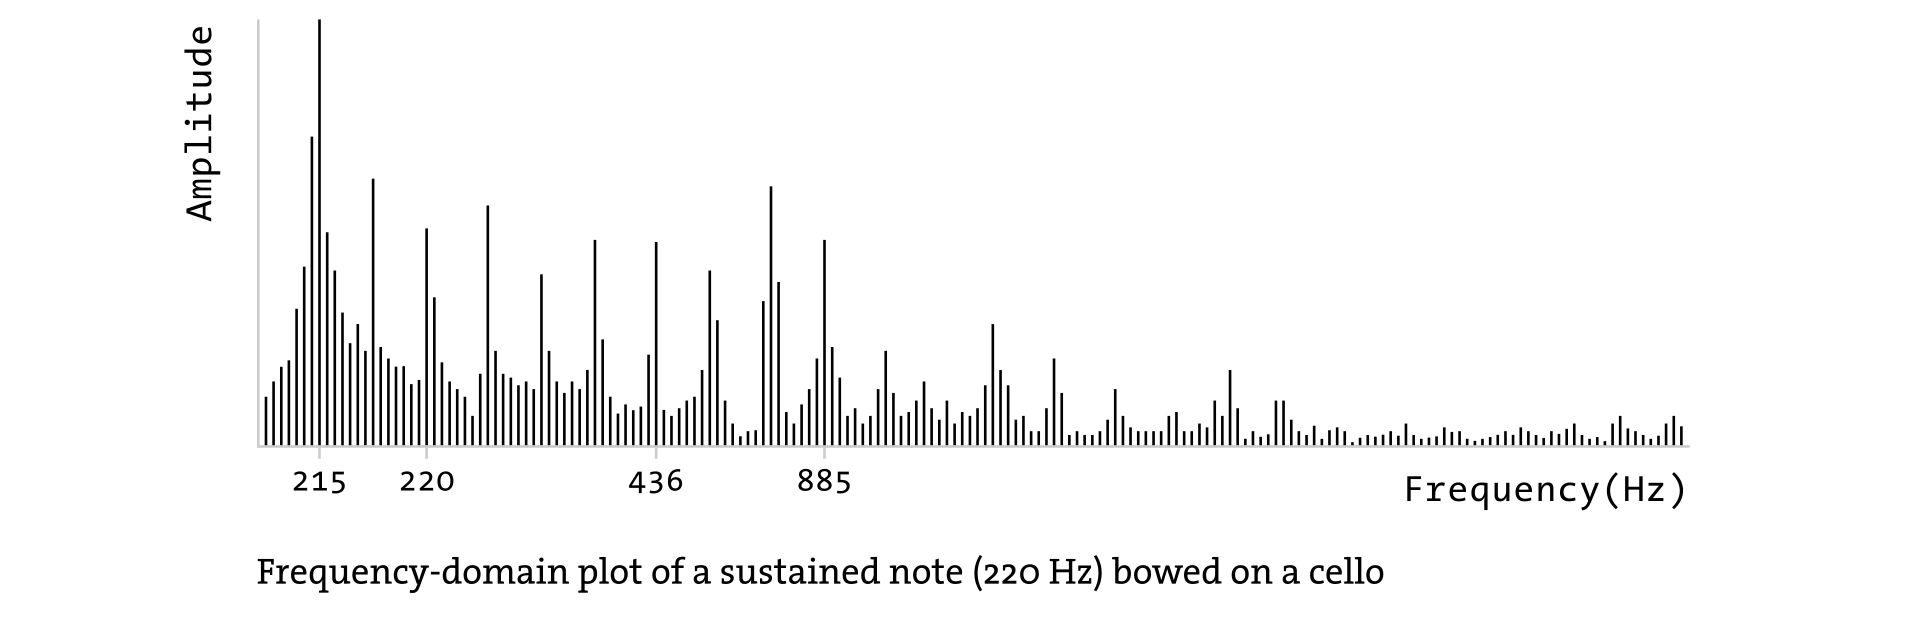
\includegraphics[scale=0.4]{img/frequency_cello.png}
\end{center}

Une fonction ou un signal donné peut être converti entre le domaine temporel et le domaine fréquentiel à l'aide d'une paire d'opérateurs mathématiques appelés transformées. Un exemple est la transformée de Fourier, qui convertit une fonction temporelle en une somme ou une intégrale d'ondes sinusoïdales de différentes fréquences, chacune d'entre elles représentant une composante de fréquence. Le "spectre" des composantes de fréquence est la représentation du signal dans le domaine des fréquences. La transformée de Fourier inverse reconvertit la fonction dans le domaine fréquentiel en fonction dans le domaine temporel. \\

\begin{center}
	\includegraphics[scale=0.22]{img/fft.png}
\end{center}

Dans le cas d'un signal numérique (ou fonction discrète) $x(t)$ la transformée de Fourier discrète sur N points est définie par :

\begin{equation}
\tcboxmath{ TFD_N( x(k) ) = X(n) = \sum_{k=0}^{N-1} x(k) \exp(-j \frac{2\pi nk}{N} ) }
\end{equation}

\vspace{0.5cm}
Ainsi la transformée de Fourier discrète inverse sur N points est définie par :

\begin{equation}
\tcboxmath{ TFD_N^{-1}( X(n) ) = x(k) = \frac{1}{N} \sum_{n=0}^{N-1} X(n) \exp( j \frac{2\pi nk}{N} ) }
\end{equation}

\vspace{0.5cm}
Les points (amplitude, fréquence) retournés par la transformée de Fourier peuvent être facilement récupérés et stocké dans une base de données. Ainsi deux signaux égaux ou correspondance entre deux musiques peut être déterminée peut être déterminé en comparant ces points deux-à-deux. Le signal stocké dans la base de données est considéré un "match" est celui qui a le plus de points (amplitude, fréquence) correspondants à celui qui est échantillonné.\\\par

\textbf{Avantages :}\\

Représentation robuste au bruit car il est devenu possible de choisir un intervalle de fréquence ou mêmes les amplitudes importantes auxquelles on applique une projection sur la base de données afin de trouver une ressemblance entre le signal enregistré via le microphone et les signaux stockés.
\\

\textbf{Inconvénients :}\\

Peu robuste à une désynchronisation et à un étirement temporel, car elle ne représente aucune évolution temporelle.

\subsection{Représentation temporelle-fréquentielle}
Un signal dans le domaine temporelle-fréquentiel est appelé \textit{Spectrogramme} et il montre les fréquences du signal et à quels moments (temps) elles sont présentes.\\
Les spectrogrammes sont largement utilisés dans les domaines de la musique, de la linguistique, des sonars, des radars, du traitement de la parole, de la sismologie, etc. Les spectrogrammes audio peuvent être utilisés pour identifier phonétiquement les mots parlés et pour analyser les différents cris des animaux.\\

\begin{center}
	\includegraphics[scale=0.45]{img/spectrogram.png}
\end{center}

Un format courant du Spectrogramme est un graphique à deux dimensions géométriques : un axe représente le temps, et l'autre axe la fréquence ; une troisième dimension indiquant l'amplitude d'une fréquence particulière à un moment donné est représentée par l'intensité ou la couleur de chaque point de l'image.\\\par

Mathématiquement pour obtenir le Spectrogramme d'un signal numérique on utilise la transformée de Fourier à court terme (STFT ou \textit{Short-Time Fourrier Transform}), il s'agit d'une séquence de transformées de Fourier du signal fenêtré. La STFT fournit les informations de fréquence localisées dans le temps pour les situations dans lesquelles les composantes de fréquence d'un signal varient dans le temps, alors que la transformée de Fourier standard fournit les informations de fréquence moyennées sur tout l'intervalle de temps du signal.\\

\begin{center}
	\includegraphics[scale=0.35]{img/stft.png}
\end{center}


Ainsi la STFT discrète sur N points est définie par :

\begin{equation}
\tcboxmath{ STFT_N(x(k)) = X(m,n) = \sum_{k=0}^{N-1} x(k)w(k-m) \exp( -j \frac{2\pi nk}{N} ) }
\end{equation}

tel que : \\

\begin{itemize}
	\item $x(k)$ est le signal d'entrée ou le signal échantillonné.
	\item $g(k)$ représente une fonction fenêtre de taille $k$ (e.g. \textit{Hanning}).
\end{itemize}

\vspace{1cm}
L'amplitude au carré de la STFT donne la représentation spectrogramme :

\begin{equation}
\tcboxmath{ spectrogram( x(k) ) = |STFT_N( x(k) )|^2 = |X(m,n)|^2 }
\end{equation}

\vspace{0.5cm}
Finalement cette représentation, \textit{temporelle-fréquentielle}, est beaucoup plus fiable par rapports aux deux représentations précédentes car elle permet d'avoir une meilleure entropie en ce qui concerne le signal échantillonné. Les points (temps, fréquence) peuvent être facilement récupérés et stocké dans une base de données. Ainsi deux signaux égaux ou correspondance entre deux musiques peut être déterminée en comparant ces points deux-à-deux. Le signal stocké dans la base de données est considéré un "match" est celui qui a le plus de points (temps, fréquence) correspondants à celui qui est échantillonné.\\\par

\newpage
\textbf{Avantages :}\\

Représentation robuste au bruit, aux distorsions, et au désynchronisation car on peut filtrer les points à très grande/basse amplitude voire appliquer d'autres filtres afin d'éliminer le bruit, sans oublier que chaque point est temporellement relatif au autres, ce qui nous aide à déterminer l'emplacement temporelle de notre échantillon à l'intérieur du signal d'origine déjà stocké dans la base de données.\\

\textbf{Inconvénients :}\\

Bien que cette représentation retourne suffisamment d'informations pour comparer avec précision deux extraits de son (deux signaux acoustiques), cette quantité d'informations pose un problème de mémoire puisqu'on doit stocker chaque point (temps, fréquence) du spectrogramme dans notre base de données, sans oublié la vitesse de comparaison entre deux signaux qui prendra beaucoup de temps si on procède par une comparaison de ces points deux-à-deux.

\section{Solution proposée et sa mise en œuvre}
Nous avons établi précédemment que le Spectrogramme est la représentation de signal qui retourne les informations nécessaires afin de résoudre les problèmes éventuels de bruits, distorsions, et désynchronisation. Donc nous avons choisi cette représentation tout en ajoutant un traitement essentiel que nous appelons \textit{Extraction des pics spectraux et constellation} afin de résoudre la problématique liée à la mémoire et à la vitesse de recherche d'un \textit{match}.\\\par
Cette une méthode qui, au lieu de traiter le spectrogramme de manière linéaire temporellement, elle se base sur une constellation de pics spectraux associés par paires. Ainsi un signal est représenté par un ensemble de paires indépendantes du point de vue temporel.\\

\begin{center}
	\includegraphics[scale=0.25]{img/constellation.png}
\end{center}

\subsection{Extraction des pics spectraux}
Un pic spectral est une paire de \textit{(temps, fréquence)} qui correspond à une amplitude localement supérieure à ses voisins (de plus forte énergie), ainsi les autres paires \textit{(temps, fréquence)} autour de ce pic spectral ont une amplitude inférieure et donc moins résistible aux bruits.\\
Premièrement on choisi une région de voisins en utilisant une structure binaire ou \textit{kernel}, dans notre application nous avons choisi la structure à 4 voisins : 

\begin{center}
	\includegraphics[scale=0.6]{img/struct.png}
\end{center}

Ceci implique qu'un pixel doit être connecté à 4 voisins de la même manière que notre structure, et il sera considéré comme un maxima local dans cette région si et seulement si sa valeur est supérieure à ses 4 voisins. Le choix de cette structure est le meilleure stratégiquement car il s'agit d'un nombre de voisins minimal ce qui implique moins de comparaisons pendant ce traitement :

\begin{center}
	\includegraphics[scale=0.6]{img/maxima.png}
\end{center}

Le nombre de voisins dans une régions est paramétrable tel que si on souhaite augmenter ce nombre on applique une ou plusieurs dilatations morphologique à notre structure par elle même ce qui étend la région de voisins, or, il faut prendre en considération que si ce nombre augmente cela implique qu'il y aura moins de maximas locaux (ou pics spectraux) à la fin de ce traitement :

\begin{center}
	\includegraphics[scale=0.6]{img/dilation.png}
\end{center}

Donc après avoir calculé le spectrogramme, nous le traitons comme une image ainsi on applique un filtre pour trouver les maximas locaux puis un deuxième filtre passe-haut pour garder seulement les amplitudes qui dépassent un seuil donné en paramètre, ce qui permet d’éliminer les maximas locaux qui varient lentement. Seule la position \textit{temps-fréquence} du pic est conservée, sans que l’amplitude soit prise en compte, afin d’obtenir directement une représentation binaire.\\\par

\newpage
Voici un exemple de cette opération réalisé sur une tableau à deux dimensions où chaque case représente une amplitude :

\begin{center}
	\includegraphics[scale=0.6]{img/peaks_explain.png}
\end{center}

Cette représentation a l’avantage d’être très robuste au bruit additif comme aux distorsions. Sans oublier une consommation minimale de la mémoire puisqu'on prend en considération que les amplitudes importantes dans notre spectrogramme.\\\par
Nous allons voir dans la partie \textit{"Création d'une empreinte acoustique"} comment nous traitons ces pics spectraux pour créer des paires indépendantes d'un point de vue temporelle, ce qui nous aidera à établir une empreinte digitale à notre signal de base qui est reproductible et éventuellement comparer deux empreinte afin de trouver rapidement un \textit{match}.

\subsection{Procédure algorithmique complète}
En guise de conclusion, le traitement du signal numérique capturé par un microphone ou directement par un fichier est une opération primordiale qui nous permettra par la suite de générer une empreinte digitale robuste au bruits, distorsions, et désynchronisation. Nous résumons ce traitement comme suit :

\begin{center}
	\includegraphics[scale=0.5]{img/dsp_algorithm.png}
\end{center}

\subsection{Mise en œuvre}
Le traitement de notre signal numérique dépend de plusieurs variables/paramètres qui contrôlent non seulement la transformée de Fourier à court terme (STFT) mais aussi la taille de la région de voisins et le seuil minimal d'amplitudes à considérer pendant l'extraction des pics spectraux.\\\par

Voici le code responsable à la création d'un \textit{Spectrogramme} à partir du signal échantillonné \textit{(channel samples)} :

\lstinputlisting[language=Python]{codes/spectrogram.py}

\vspace{1cm}
Voici le code responsable à l'\textit{Extraction des Pics Spectraux} en utilisant un traitement d'image sur le \textit{Spectrogramme} du signal échantillonné :

\lstinputlisting[language=Python]{codes/peaks.py}


\section{Tests et certifications de la solution}
Dans cette partie nous allons effectuer des tests sur un signal échantillonné à travers un fichier mp3 qui s'agit d'une musique intitulée \textit{"Know yourself - Drake"}. Nous allons aussi prendre en considération, que pour ce test, qu'un seul canal pour démontrer le fonctionnement du traitement du signal, par contre notre application traite les deux canaux séquentiellement.\\\par

Il est nécessaire de prendre en considération tous les paramètres de notre application que nous avons définie précédemment dans le code, et qui influencent directement sur la qualité du résultat final ainsi sur le temps d'exécution.\\\par
Pour notre application nous choisissons les valeurs suivantes pour nos paramètres :\\

\begin{itemize}
	\item Fréquence d'échantillonnage (FS) = 44100
	\item Taille de la fenêtre utilisée dans la fonction STFT (WINDOW SIZE) = 4096
	\item Ratio du chevauchement des fenêtres consécutive (OVERLAP RATIO) = 0.5 (la moitié)
	\item Seuil d'amplitude minimale pour être considérée comme un pic spectral (AMP MIN) = 10
	\item Taille de la région des voisins utilisée dans la recherche des maximas locaux (NEIGHBORHOOD SIZE) = 20
\end{itemize}

\vspace{0.5cm}
La musique dure 277 secondes (4 minutes 37 secondes), ainsi avec une fréquence d'échantillonnage égale à 44100 nous enregistrons 44100 points d'entrée pour chaque secondes, ce qui implique que nous signal échantillonné est de taille :

\begin{equation}
\tcboxmath{ Digital Signal Size = duration \times FS =  277 \times 44100 = 12 215 700 }
\end{equation}

\vspace{0.5cm}
Comme expliqué dans le code, chacun de ces paramètre influence directement sur le nombres des pics spectraux retourner à la fin du traitement voire aussi sur le temps de ce traitement.\\
Nous avons expérimenté avec différentes valeurs ainsi nous avons choisi celles-ci par comparaison de résultats.\\
Il ne s'agit pas des valeurs optimales, il se peut qu'il existe une meilleure approche, or il est difficile de mettre en place un protocole assez profond afin de trouver des valeurs optimales car cela prendra énormément de temps pour le réaliser.\\
On peut citer comme protocole la mise en place d'un réseaux neurones qui prends en entrée tous les paramètres de notre application du traitement du signal et l'entraîner sur une large base de tests qu'on peut effectuer, ainsi ce réseaux pourra déterminer des valeurs qui se rapprochent à l'optimal pour un résultat souhaité.

\newpage
\subsection{Tests préliminaires}
Les tests suivants ne comportent aucun bruit ajouté sur le signal d'origine. \\\par
Voici le résultat retourner par la fonction \textit{get\_spectrogram} :\\

\begin{center}
	\includegraphics[scale=0.535]{img/spectrogram_drake.png}
\end{center}

Maintenant nous allons extraire les pics spectraux ainsi construire une carte de constellation en utilisant la fonction \textit{get\_peaks} : \\

\begin{center}
	\includegraphics[scale=0.5]{img/constallation_drake.png}
\end{center}

Pour les deux opérations nous avons :

\begin{center}
	\begin{tabular}{ | m{3cm} || m{4cm}| m{4cm} | } 
		\hline
		operation & execution time (sec) & output size \\ 
		\hline
		\hline
		spectrogram & 0.91859579 & 12169011 \\ 
		\hline
		peaks extraction & 11.18466210 & 6128 \\ 
		\hline
	\end{tabular}
\end{center}

On remarque que la création d'un \textit{Spectrogramme} prend un temps négligeable par rapport à l'extraction des pics spectraux (avec la taille de région de voisin égale à 20). Or, la réduction de la taille finale est considérablement bénéfique car nous avons économisé $99.95\%$ de mémoire en choisissant les amplitudes importantes dans notre signal numérique.

\newpage
Si on augment le nombre de voisins à prendre considération lors de l'identification des maximas locaux alors le nombre des pics spectraux diminuera considérablement, voici un exemple pour une valeur $NEIGHBORHOOD\_SIZE = 50$ :

\begin{center}
	\includegraphics[scale=0.5]{img/constallation_drake_50.png}
\end{center}

Pour les deux opérations nous avons :

\begin{center}
	\begin{tabular}{ | m{3cm} || m{4cm}| m{4cm} | } 
		\hline
		operation & execution time (sec) & output size \\ 
		\hline
		\hline
		spectrogram & 0.90590810 & 12169011 \\ 
		\hline
		peaks extraction & 69.41175055 & 987 \\ 
		\hline
	\end{tabular}
\end{center}

Nous économisons encore plus de mémoire, or, le temps de traitement augmente drastiquement. Sans oublier que le nombre final des pics spectraux influence sur la précision de l'identification d'un \textit{match}, ainsi elle sera moins précis si on réduit beaucoup le nombre des pics spectraux.

\subsection{Tests de robustesse de la constellation}
Dans cette partie nous allons effectuer une série de tests sur la même musique tout en rajoutant différents types de distorsions. Nous utilisons les même paramètres de l'application cités précédemment.

\subsubsection{Bruit réel : groupe de gens dans un bar}
Nous avons rajouté un bruit au-dessus notre musique originale qui s'agit d'un groupe de gens qui parlent dans un bar tout en contrôlant l'intensité (loudness) de ce bruit.
Cette intensité est exprimé en \textit{dBFS} (Decibels relative to Full Scale), il s'agit d'une unité de niveau de signal audio. Elle indique le rapport entre le niveau de ce signal et le niveau maximal qui est 0 dBFS.\\
Comme un premier test nous allons rajouté le bruit en question avec une intensité de -17.23 dBFS, ainsi peut directement visualiser les changements du signal qui résulte de l'ajout de notre bruit réel sur le \textit{Spectrogramme} :

\begin{center}
	\includegraphics[scale=0.535]{img/spectrogram_drake.png}\vspace{1cm}
	\includegraphics[scale=0.535]{img/spec_drake_crowd.png}
\end{center}


Comme on peut aussi voir les changements après l'extraction des pics spectraux, nous allons voir que le nombre de pics augmente tout en rajoutant plus d'intensité à notre bruit :

\begin{center}
	\includegraphics[scale=0.5]{img/constallation_drake.png}\vspace{1cm}
	\includegraphics[scale=0.5]{img/peaks_drake_crowd.png}
\end{center}

\newpage
Si on superpose les deux constellations précédente nous allons voir les points différents et aussi les points similaires entre le signal original et le signal bruité :

\begin{center}
	\includegraphics[scale=0.5]{img/similitude_drake_crowd.png}
\end{center}

Focalisons nous sur une petite région afin de mieux voir la différence et la similitude :

\begin{center}
	\includegraphics[scale=0.5]{img/similitude_drake_crowd_zoom.png}
\end{center}

On remarque bien que l'union des deux constellation n'est pas disjointe et qu'il existe des points en commun entre les deux signaux. Ceci implique que notre approche au traitement du signal numérique est bien robuste au bruit additif.\\

Voici un tableau qui montre plus de détails sur cette similitude tout en augmentant l'intensité du bruit :

\begin{center}
	\begin{tabular}{ | m{3cm} || m{3cm}| m{3cm} | m{5cm} | } 
		\hline
		source (mp3) & loudness (dBFS) & output size & similitude with original (\%) \\ 
		\hline
		\hline
		original & -12.99 & 6128 & 100  \\ 
		\hline
		crowd noise & -37.23  & 5840 & 58.44  \\ 
		\hline
		crowd noise & -27.27 & 6088 & 51.23  \\ 
		\hline
		crowd noise & -17.23 & 6593 & 38.12  \\ 
		\hline
		crowd noise & -7.50 & 7806 & 16.44  \\ 
		\hline
	\end{tabular}
\end{center}

\subsubsection{Bruit additif blanc Gaussien}
Dans ce test nous allons rajouter du bruit blanc Gaussien à notre signal original. Le bruit additif blanc Gaussien est un modèle élémentaire de bruit utilisé en théorie de l'information pour imiter de nombreux processus aléatoires qui se produisent dans la nature. Les adjectifs indiquent qu'il est :\\

\begin{itemize}
	\item \textbf{additif} : il s'ajoute au bruit intrinsèque du système d'information;
	\item \textbf{blanc} : sa puissance est uniforme sur toute la largeur de bande de fréquences du système, par opposition avec un bruit coloré qui privilégie une bande de fréquences par analogie avec une lumière colorée dans le spectre visible; 
	\item \textbf{gaussien} : il a une distribution normale dans le domaine temporel avec une moyenne nulle.
\end{itemize}

\vspace{0.5cm}
Comme un premier test nous allons rajouté le bruit en question avec une intensité de -24.76 dBFS, ainsi peut directement visualiser les changements du signal qui résulte de l'ajout de notre bruit gaussien sur le \textit{Spectrogramme} et sur la \textit{Constellation}, sans oublier les points communs entre les deux signaux :

\begin{center}
	\includegraphics[scale=0.535]{img/spec_drake_wn.png}\vspace{1cm}
	\includegraphics[scale=0.5]{img/peaks_drake_wn.png}\vspace{1cm}
	\includegraphics[scale=0.5]{img/similitude_drake_noise_zoom.png}
\end{center}

Voici un tableau qui montre plus de détails sur cette similitude tout en augmentant l'intensité du bruit gaussien :

\begin{center}
	\begin{tabular}{ | m{4cm} || m{3cm}| m{3cm} | m{5cm} | } 
		\hline
		source (mp3) & loudness (dBFS) & output size & similitude with original (\%) \\ 
		\hline
		\hline
		original & -12.99 & 6128 & 100  \\ 
		\hline
		gaussian white noise & -34.77  & 7162 & 47.88  \\ 
		\hline
		gaussian white noise & -24.76 & 8200 & 32.31  \\ 
		\hline
		gaussian white noise & -14.77 & 9681 & 15.93  \\ 
		\hline
	\end{tabular}
\end{center}

\vspace{0.5cm}
On peut observer ce qui suit :\\
\begin{itemize}
	\item Les cartes de constellations des versions déformées partagent plusieurs pics avec la version originale.
	\item Les pics des versions déformées sont parfois légèrement décalés en temps et/ou en fréquence par rapport à ceux de la version originale.
\end{itemize}

\vspace{0.5cm}
Le nombre de points de correspondance sera significatif en présence de pics parasites injectés en raison du bruit, car les positions des pics sont relativement indépendantes; en outre, le nombre de correspondances peut également être significatif même si de nombreux points corrects ont été supprimés. L'enregistrement des cartes de constellation est donc un moyen puissant d'établir des correspondances en présence de bruit et/ou de suppression de caractéristiques. Cette procédure réduit le problème de recherche à une sorte d'\textit{astronavigation}, dans laquelle une petite parcelle de points de constellation de fréquence-temps doit être rapidement localisée dans un grand univers de constellations.\\

Nous allons voir par la suite comment ces pics spectraux peuvent être utilisés afin de créer une empreinte digitale au signal d'entrée et à quel point cela influence sur la vitesse/robustesse de la recherche d'une correspondance.

\chapter{Création d'une empreinte acoustique}
\label{hash}
Après avoir converti le signal numérique à un \textit{Spectrogramme} puis le traiter pour extraire les pics spectraux, nous allons voir comment utiliser ces pics afin de produire une empreinte digitale de ce signal.\\

Une empreinte audio est un résumé numérique qui peut être utilisé pour identifier un échantillon audio. Cette empreinte permet de localiser rapidement des éléments similaires dans une base de données audio.\\\par

Dans ce chapitre nous allons présenter les problématiques liées à l'utilisation directe des pics spectraux et pourquoi nous avons besoin de les représenter différemment, ainsi le processus de création d'une empreinte qui est basé principalement sur la construction des paires de pics.\\

\section{Analyse de la problématique}

A ce niveau nous avons les pics de notre signal audio, ces pics peuvent être des milliers pour une seule musique. Ils caractérisent très bien notre signal, or comment ils peuvent être utilisé pour créer une empreinte digitale à notre audio tout en respectant la définition (conditions) d'une empreinte ? \\

Il reste à retrouver dans cette masse d’empreintes, la centaine d’empreintes obtenues à partir de la musique enregistrée depuis notre microphone.\\
Puisque les empreintes tirées de l’échantillon sont bruitées, il faut comparer une centaine d’empreinte qui vont chacune correspondre à plusieurs morceaux, donc on se retrouvera avec beaucoup de morceaux potentiellement candidats.\\\par

Une empreinte acoustique doit satisfaire plusieurs conditions :\\

\begin{itemize}
	\item \textbf{Spécificité} : L'empreinte doit être assez précise pour que deux sons très différents n'aient pas la même empreinte.
	\item \textbf{Robustesse aux les distorsions} : Un algorithme d'empreinte acoustique doit tenir compte des caractéristiques audibles du son.\par
	Si deux échantillons sont perçus comme identiques par l'oreille humaine, leur empreinte doit être égale ou très proche, même si leur représentation numérique est différente. À ce titre les empreintes acoustiques ne sont pas des empreintes au sens habituel du terme.\\
	Un bon algorithme d'empreinte acoustique va permettre d'identifier un enregistrement même après qu'il a subi une compression, une légère variation de vitesse ou un bruit léger doit aussi ne pas trop changer l'empreinte.
	\item \textbf{Efficacité} : Pour être utilisée, l'empreinte doit être facile à calculer, et facile à stocker, c'est-à-dire compacte, courte.\\
\end{itemize}

Sans oublier la problématique de l'alignement des empreintes. Si l'enregistrement à partir du microphone de l'ordinateur n'est pas commencé depuis le début de la musique alors les empreintes enregistrée à partir du microphone ne vont pas s'alignés correctement avec ceux obtenus à partir de la base de données.\\

\section{État de l’art : études des solutions existantes}
Dans cette partie, nous allons présenter deux approches qui amènent à résoudre ces problématiques tout en précisant les avantages et les inconvénients de chaque représentations.\\\par

\subsection{Approche de superposition}
Les pics spectraux caractérisent très bien notre signal, ils sont assez spécifiques, robuste au bruit et aux distorsions et plus ou moins efficace, ainsi ils peuvent être explicitement considérés comme une empreinte de notre signal.\\

Ce que nous voulons dire par cela c'est que nous allons stocker directement les pics spectraux ou les points \textit{(temps, fréquence)} dans notre base de données, ainsi lors d'une recherche de correspondance, nous allons comparer ces pics deux-à-deux.\\

Il est plus simple d'imaginer ce processus comme une superposition de la carte de constellation du signal enregistré à travers le microphone et celle du signal enregistré dans la base de données.\\
Le pattern des points doit être le même pour les segments audio correspondants. Si vous mettez la carte des constellations d'une
chanson de la base de données sur un ruban, et la carte de constellation de d'un court échantillon audio de quelques secondes sur un morceau de ruban transparent, puis vous glissez le second sur le premier, à un moment donné, un nombre significatif de points coïncideront lorsque le décalage temporel adéquat sera trouvé et que les deux cartes de constellation seront alignées.\\

\begin{figure}[H]
	\centering
	\includegraphics[scale=0.52]{img/superposition.png}
	\caption{Original Track and Recording Constellations}
\end{figure}

\begin{figure}[H]
	\centering
	\includegraphics[scale=0.6]{img/superposition_process.png}
	\caption{Superposition Process}
\end{figure}

Dans cet exemple, il y a une correspondance parfaite entre l'enregistrement et la fin de la chanson.\\
Si ce n'est pas le cas, nous devons comparer l'échantillon avec une d'autre chansons dans la base de données et ainsi de suite jusqu'à ce qu'on trouve une correspondance parfaite.\\
Et si on ne trouve pas de correspondance parfaite, nous pouvons choisir la correspondance la plus proche que nous avons trouvée (dans toutes les chansons) si le taux de correspondance est supérieur à un seuil qui pourra être fixé en paramètre.\\
Par exemple, si la meilleure correspondance que nous avons trouvée nous donne une similitude de 90\% entre le segment échantillon et une partie d'une chanson, nous pouvons supposer que c'est un \textit{match} car les 10\% de non-similitude sont certainement dus aux distorsions et au bruit.\\

\textbf{Avantages :}\\

Il s'agit d'une solution directe, aucun traitement supplémentaire sur les cartes de constellation. On les enregistre directement dans la base de données et on les compare tout en respectant la séquentialité temporelle pour un bon alignement.\\

\textbf{Inconvénients :}\\

Bien que les pics spectraux sont résistants au bruit et aux distorsions,  \textbf{individuellement} \footnote{pour éviter une contradiction avec ce qu'on a dit au début de cette section.} ils ont une faible spécificité, cela veut dire qu'ils ne sont pas très caractéristiques lorsqu'ils sont considérés de manière isolée. Par conséquent, lorsqu'on utilise des pics spectraux individuels et leurs timbres de fréquence comme valeurs de hachage, alors les listes de hachage résultantes (la liste des numéros de page) sont longues et l'indexation devient lente.\\

\subsection{Approche de hachage combinatoire}

L'idée principale est de former des hachages d'empreintes digitales en considérant des paires de pics plutôt que des pics individuels. Pour cela, on fixe un point $(n_0,k_0)$ qui sert de point d'ancrage ainsi qu'une zone cible $Z \times$ qui lui est associée. La zone cible doit être considérée comme une petite région rectangulaire dans le plan temps-fréquence proche du point d'ancrage. On considère alors des paires de points $((n_0,k_0),(n_1,k_1))$ constitués du point d'ancrage $(n_0,k_0)$ et d'un certain point cible $(n_1,k_1) \in Z$. Chaque paire donne lieu à un triplet $(k_0,k_1,n_1-n_0)$ constitué de deux estampilles de fréquence et d'une différence de deux estampilles de temps. L'idée est d'utiliser ces triplets comme des hachages au lieu d'estampilles de fréquence simples.\\

\begin{figure}[H]
	\centering
	\includegraphics[scale=0.3]{img/hash_comb.png}
	\caption{Combinatorial Hash Generation}
\end{figure}


Au stade de la mise en correspondance, on compte maintenant les triples correspondances entre la requête décalée et le document de la base de données au lieu de considérer uniquement les timbres de fréquence correspondants. On peut montrer que, même si le nombre d'éléments de données à indexer augmente (en considérant les triples au lieu des timbres de fréquence simples), on obtient une accélération considérable du processus de recherche grâce à la grande spécificité beaucoup des triples.\\

\newpage
\textbf{Avantages :}\\

Cette solution permet de gagner une accélération dans la recherche d'une correspondance, sans oublier que les paires spectraux sont indépendants du points de vue temporelle c'est à dire un paire $ (k_0,k_1,\Delta t_0) $ est indépendant temporellement du paire $ (k_2,k_3,\Delta t_2) $ et ainsi de suite, ce qui rend la comparaison entre les paires plus simple voire plus robuste.\\

\textbf{Inconvénients :}\\

Ce processus consiste à itérer sur les pics spectraux, chaque pics sera considéré comme un point d'ancrage et associé à une zone cible puis itérer sur cette zone pour construire les paires à trois valeurs $(k_0,k_1,\Delta t_0)$ : 2 valeurs de fréquence absolues et 1 valeur de différence temporelle. Donc on peut facilement conclure que ce processus peut générer une quantité immense de données en fonction de la taille de la zone cible, ce qui pourra poser des problématique du point de vue de mémoire.

\section{Solution proposée et sa mise en œuvre}

D'après l'étude des solutions existantes réalisée précédemment, nous avons choisi d'implémenter la solution du \textit{Hachage Combinatoire} afin de construire les empreintes digitale de n'importe quel signal d'entrée. Bien que celle-ci posera un défi du point de vue de mémoire, nous allons voir par la suite comment nous allons optimiser l'espace qui sera occupé par le nombre immense d'empreintes.\\

La procédure du \textit{Hachage Combinatoire} ce réalise en passant par deux étapes cruciales :\\

\begin{itemize}
	\item Construction des paires en utilisant les zones cibles.
	\item Conversion des repères en valeurs de hachage.
\end{itemize}	

\subsection{Construction des paires}
Nous choisissons une zone cible en fonction des voisins, c'est à dire pour un point d'ancrage $k$, nous allons choisir un nombre fini de points à son voisinage, ce nombre est défini en paramètre de notre application.

\begin{figure}[H]
	\centering
	\includegraphics[scale=0.3]{img/pairs.png}
	\caption{Pairs Connections}
\end{figure}

\begin{figure}[H]
	\centering
	\includegraphics[scale=0.45]{img/anchor_point.png}
	\caption{Anchor Point and Target Zone}
\end{figure}


A partir d'un point donné, ses voisins sont choisit en fonction de leur distance, c'est à dire les points les plus proches temporellement.   

Par souci de compréhension, nous fixerons la taille de la zone cible à 5 points temps-fréquence.\\
Afin d'être sûr que l'enregistrement et le morceau complet généreront les mêmes zones cibles, nous avons besoin d'une relation d'ordre entre les points (temps-fréquence) dans un spectrogramme filtré :\\

\begin{itemize}
	\item Si deux points (temps,fréquence) ont le même temps, le point avec la fréquence la plus basse est avant l'autre.
	\item Si un point (temps,fréquence) a un temps inférieur à un autre point, alors il est avant.
\end{itemize} 

\vspace{0.5cm}
Voici ce que nous obtenons si nous appliquons cet ordre sur le \textit{Spectrogramme} simplifié que nous avons vu précédemment:

\begin{figure}[H]
	\centering
	\includegraphics[scale=0.62]{img/pairs2.png}
	\caption{Pairs Order}
\end{figure}

\vspace{0.5cm}
On associe à chacun des pics extraits (les points ancres, anchor points) une zone cible (target zone). La taille de la zone cible influe directement sur le nombre de paires résultant.\\
À chaque \textit{anchor} point est associée sa position temporelle par rapport au début du signal, et chaque paire \textit{ \{anchor point,target point\}} est codée par 3 valeurs $(f1, f2, \Delta t)$ : 2 valeurs de fréquence absolues et 1 valeur de différence temporelle. Ces couples sont formés de trois éléments:\\

\begin{itemize}
	\item la fréquence du point d’ancrage ($f1$)
	\item la fréquence du point de la zone cible ($f2$)
	\item la différence de temps entre les deux ($\Delta t$).
\end{itemize}

\vspace{0.5cm}
Nous allons voir par la suite comment nous allons convertir cette représentation de triplet à un hache reproductible et simple à stocker.

\subsection{Conversion des repères en valeurs de hachage.}

Le hachage est Opération qui consiste à appliquer une fonction mathématique permettant de créer l'empreinte numérique d'un message, en transformant un message de taille variable en un code de taille fixe, en vue de son authentification ou de son stockage.\\

Une fonction de hachage est typiquement une fonction qui, pour un ensemble de très grande taille (théoriquement infini) et de nature très diversifiée, va renvoyer des résultats aux spécifications précises (en général des chaînes de caractère de taille limitée ou fixe) optimisées pour des applications particulières. Les chaînes permettent d'établir des relations (égalité, égalité probable, non-égalité, ordre...) entre les objets de départ sans accéder directement à ces derniers, en général soit pour des questions d'optimisation (la taille des objets de départ nuit aux performances), soit pour des questions de confidentialité.\\
En termes très concrets, on peut voir une fonction de hachage comme un moyen de replier l'espace de données que l'on suppose potentiellement très grand et très peu rempli pour le faire entrer dans la mémoire de l'ordinateur.\\\par

Après avoir formé des paires de points \textit{ \{anchor point,target point\}} comme décrit avant, et que nous les avons encodé par 3 valeurs $(f1, f2, \Delta t)$ : 2 valeurs de fréquence absolues et 1 valeur de différence temporelle, tel que :\\

\begin{itemize}
	\item la fréquence du point d’ancrage ($f1$)
	\item la fréquence du point de la zone cible ($f2$)
	\item la différence de temps entre les deux ($\Delta t$).
\end{itemize}

\vspace{0.5cm}
Ensuite nous avons choisi la fonction SHA-1 afin de hacher ces 3 valeurs.
Ces haches sont tout à fait reproductibles, même en présence de bruit et de la compression du codec vocal.\\

\begin{lstlisting}[language=C]
hash(frequencies of peaks, time difference between peaks) = fingerprint hash value
\end{lstlisting}

\vspace{0.5cm}
Chaque hachage est également associé au décalage temporel entre le début du fichier respectif et son point d'ancrage, ce que nous appelons dans notre application un \textit{offset}. Bien que le temps absolu ne fasse pas partie du hachage lui-même. 

\begin{figure}[H]
	\centering
	\includegraphics[scale=0.45]{img/hash_algo.png}
	\caption{Combinatorial Hash Function}
\end{figure}

Ce couple est ce que l’on appelle un \textit{marqueur}. On assigne ensuite à ce \textit{marqueur} l’instant $t$ du point d’ancrage pour obtenir un \textit{marqueur temporel}. Le regroupement de tous les marqueurs temporels forme l’empreinte.\\

A cette empreinte, on associera par la suite les informations du morceau (artiste, nom de la chanson, etc). En moyenne, une empreinte se retrouve dans seulement trois morceaux.\\
Pour effectuer une recherche, l'étape d'empreinte digitale ci-dessus est exécutée sur un échantillon de fichier sonore capturé pour générer un ensemble de \textit{[hache : offset]}. Chaque hachage de l'échantillon est utilisé pour rechercher dans la base de données les haches correspondants. Pour chaque haches correspondant trouvé dans la base de données, les temps de décalage ou \textit{offset} correspondants depuis le début de l'échantillon et les fichiers de la base de données sont associés en paires de temps. Les paires de temps sont distribuées dans des bacs en fonction de l'ID de la musique associée au hache correspondant dans la base de données.\\

Nous allons voir dans le chapitre \textit{Base de données : stockage et recherche}, en détails, la procédure de recherche et le nombre d'empreintes généré pour une collections de 50 musiques ainsi étudier la problématique de mémoire et voir comment on pourra optimiser l'espace occupé par les haches.

\chapter{Base de données: stockage et recherche}
\label{bdd}
Récapitulons ce que nous avons réalisé jusqu'à maintenant :\\

\begin{enumerate}
	\item Nous avons d'abord capturer le signal en utilisant le microphone et avec une fréquence d'échantillonnage égale à 44 100 Hz.
	\item Une fois le signal est numérisé, nous appliquons la fonction \textit{Short-Time Fourier Transform (STFT) } afin de passer d'une représentation temporelle simple à une représentation fréquentielle-temporelle et générer un \textit{Spectrogramme} du signal.
	\item Ensuite nous avons appliqué un filtre pour extraire les maximas locaux de ce \textit{Spectrogramme} et un deuxième filtre pour garder seulement les amplitudes qui dépassent un certain seuil. Ceci nous donne les pics spectraux du signal, ou en autres mots les amplitudes importantes du signal qui résistent aux bruits et autres distorsions. Bien-sur nous gardons seulement le couple \textit{(temps, fréquence)} associé à chaque pic spectral comme ça on aura une représentation binaire. 
	\item Après nous avons vu qu'au lieu de stocker directement les couples \textit{(temps, fréquence)} des pics spectraux directement dans une base de données puis comparer les points deux-à-deux afin de trouver une correspondance entre deux signaux, nous formons des paires de points en choisissons un point d'ancrage et une zone cible, puis on garde les fréquences du point d'ancrage et du point cible voir aussi la différence temporelle entre ces deux points, ce qui nous donne une représentation plus compacte et suffisamment informative qui pourra être facilement stocker.
	\item Finalement nous utilisons SHA-1 pour hacher cette représentation ainsi créer une empreinte digitale du signal d'entrée ce qui rend la recherche/comparaison plus simple voire plus rapide.
\end{enumerate}

\vspace{0.5cm}
Tous ces éléments réunis nous donne la possibilité de mettre en œuvre une reconnaissance de musique car un tel système doit réaliser deux taches principales : \\

\begin{enumerate}
	\item Apprendre de nouvelles chansons en enregistrons leurs empreintes digitales.
	\item Reconnaître des chansons inconnues en les recherchant dans la base de données des chansons déjà apprises.
\end{enumerate}

\vspace{0.5cm}
Alors dans ce chapitre nous allons voir comment nous avons traité le côté base de données (tables, contraintes sur des champs, indexation...) afin de stocker une large quantité de données tout en permettant une recherche rapide qui ne dépasse pas 1 seconde pour trouver un \textit{match}.

Certes qu'après l'extraction des points importants du \textit{Spectrogramme} du signal puis le hachage combinatoire de ces points, nous diminuons largement la quantité de données à stocker. Néanmoins, cette quantité reste quand même très large car nous obtenons des milliers de haches par signal, donc si nous appliquons une extrapolation sur une collection de 8411 musiques mp3 à hacher et à stocker, alors il est clair que notre base de données contiendra des millions voire des milliards d'articles (lignes). Ceci nous oblige à étudier la façon dans laquelle nous allons créer nos tables ainsi l'architecture globale de notre base de données afin de permettre une fouille très rapide pour trouver un \textit{match}.\\\par

Nous avons donc étudié deux approches de mise en place de la base de données, dans ces deux approches nous aurons que deux tables, or, il y aura une différence très importante quand il s'agit des champs et des contraintes.

\section{Architecture initiale de la base de données}
Il s'agit d'une approche simple qui ne prend aucune considération de la complexité en mémoire et en temps de recherche. Nous avons choisi de parler de cette architecture afin d'accentuer le niveau d'optimisation atteint dans notre application et aussi pour montrer que des petites modification dans les contraintes des champs peut avoir un grand impacte sur les performances de la base de données. 

\subsection{Mise en œuvre}
Commençant d'abord par la table \textbf{SONGS}, nous l'utiliserons essentiellement pour contenir des informations sur les chansons. Nous en aurons besoin pour associer un song\_id à la chaîne de caractères du nom de la chanson. :\\

\lstinputlisting[language=SQL]{codes/songs_table.sql}

\vspace{0.5cm}
Cette table ne change pas dans les deux architectures que nous étudions. Or, la vrai différence est sera dans la deuxième table intitulée \textbf{FINGERPRINTS}, dans cette première approche la table est crée comme suit :\\

\lstinputlisting[language=SQL]{codes/fingerprints_table1.sql}

\vspace{0.5cm}
Tout d'abord, remarquez que nous avons non seulement champ \textit{hash} et un identifiant \textit{song\_id}, mais aussi un \textit{offset}. Celui-ci correspond à la fenêtre temporelle du \textit{Spectrogramme} d'où provient le hachage. Cela entrera en jeu lorsque nous devrons filtrer les haches correspondants pendant la recherche. Seuls les haches qui "s'alignent" proviendront du véritable signal que nous voulons identifier.
En supposant que nous avons déjà crée des empreintes digitales des pistes connues, c'est-à-dire que nous avons déjà inséré nos empreintes digitales dans la base de données étiquetée avec les ID des chansons, nous pouvons simplement chercher un \textit{match}.\\

Notre pseudo-code pour une recherche d'un match sera écrit comme suit :

\lstinputlisting[language=Python]{codes/search_match.py}

\vspace{0.5cm}
Qu'est-ce que cela signifie pour les hachages d'être alignés ? Considérons l'échantillon que nous écoutons comme un sous-segment de la piste audio originale. Une fois que nous avons fait cela, les hachages que nous extrayons de l'échantillon auront un décalage relatif au début de l'échantillon.\\

Le problème, bien sûr, est que lorsque nous avons crée les empreintes digitales des pistes originales \textit{mp3}, nous avons enregistré le décalage absolu du hachage. Les hachages relatifs de l'échantillon et les hachages absolus de la base de données ne correspondront jamais, sauf si nous avons commencé à enregistrer un échantillon exactement au début de la chanson. Assez peu probable.\\

Mais même si elles ne sont pas identiques, nous avons une idée sur les correspondances à partir du signal réel derrière le bruit. Nous savons que tous les décalages relatifs seront à la même distance les uns des autres. Bien-sur il faut que la chanson est lue et échantillonnée à la même vitesse qu'elle a été enregistrée pendant la création des empreintes (44 100 Hz).\\
Dans cette hypothèse, pour chaque correspondance, nous calculons une différence entre les décalages :\\

\begin{lstlisting}[language=C]
difference = database offset from original track - sample offset from recording
\end{lstlisting}

\vspace{0.5cm}
Ce qui donnera toujours un entier positif puisque la chanson de la base de données sera toujours au moins de la même longueur de l'échantillon. Toutes les vraies correspondances auront cette même différence. Ainsi, nos correspondances de la base de données sont modifiées pour ressembler à ceci : \\

\begin{lstlisting}[language=C]
(song_id, difference)
\end{lstlisting}

\vspace{0.5cm}
Maintenant, il suffit de regarder toutes les correspondances et de prédire l'identifiant de la chanson pour laquelle le nombre de différences est le plus élevé. C'est facile à imaginer si vous le visualisez sous forme d'histogramme.\\

\subsection{Tests et performance}
Maintenant que notre base de données est prête à être utilisée, nous allons choisir les même paramètres qu'avant quand il s'agit du traitement de signal et qui sont : \\

 \begin{itemize}
 	\item Fréquence d'échantillonnage (FS) = 44100
 	\item Taille de la fenêtre utilisée dans la fonction STFT (WINDOW SIZE) = 4096
 	\item Ratio du chevauchement des fenêtres consécutive (OVERLAP RATIO) = 0.5 (la moitié)
 	\item Seuil d'amplitude minimale pour être considérée comme un pic spectral (AMP MIN) = 10
 	\item Taille de la région des voisins utilisée dans la recherche des maximas locaux (NEIGHBORHOOD SIZE) = 20
 	\item Taille de la zone cible pour chaque point d'ancrage (FAN VALUE) = 15
 \end{itemize}

\vspace{0.5cm}
Ensuite nous allons utiliser 50 chansons mp3 afin de peupler notre base de données avec leurs empreintes digitales ainsi étudier la taille de mémoire occupée et la temps de recherche d'un \textit{match}.\\

Voici un tableau qui montre le nombre de lignes dans chaque tables ainsi que sa taille totale :

\begin{center}
	\begin{tabular}{ | m{3.5cm} || m{3cm}| m{3cm} | m{3cm} | m{3cm} | } 
		\hline
		table & number of lines & data size (Mo) & index size (Mo) & total size (Mo) \\ 
		\hline
		\hline
		SONGS & 50 & 0.016 & 0.016 & 0.016 \\ 
		\hline
		FINGERPRINTS & 9 681 644 & 702.0 & 116.7 & 818.7 \\ 
		\hline
	\end{tabular}
\end{center}

On remarque bien que même après extraction de pics le nombre d'empreintes est immense, 9 681 644 empreintes pour seulement 50 musiques. On peut imaginer ce nombre atteindre des milliards voire même plus si on rajoute d'autres musiques à notre base de données.\\

\newpage
Voici un graphique qui montre la nombre d'empreintes (ou hache) pour chaque musique dans la base de données : \\

\begin{figure}[H]
	\centering
	\includegraphics[scale=0.55]{img/histogram1.png}
	\caption{Bar chart representing the number of fingerprints by song}
\end{figure}

\vspace{0.5cm}
Ce graphique montre la grandeur que notre application peut atteindre en terme de mémoire, puisqu'on peut bien avoir des musiques avec un nombre d'empreintes qui dépasse 300 000, et que la moyenne dépasse 100 000.\\\par

Il faut aussi retenir que ce nombre est un résultat direct des pics du signal, et que le nombre de pics peut diminuer si on change les paramètres cités au début. Ceci résultera une décroissance dans le nombre d'empreintes ainsi moins d'espace occupé. Or, moins d'empreintes signifie moins de précision. Donc il faut absolument réaliser une étude approfondie pour trouver les paramètres optimales en terme de mémoire et de précision.\\
En même temps il faut se demander si il existe un moyen pour optimiser la mémoire, même avec une petite marge, sans changer les paramètres.


\section{Optimisation de la base de données}
Comme décrit avant, la table \textbf{SONGS} ne changera pas. Néanmoins nous allons voir des améliorations non négligeable en changeant la table \textbf{FINGERPRINTS}.

\subsection{Mise en œuvre}
Dans cette deuxième approche la table \textbf{FINGERPRINTS} est crée comme suit : \\

\lstinputlisting[language=SQL]{codes/fingerprints_table2.sql}

\vspace{0.5cm}
Nous avons créé un INDEX sur notre champs \textit{hash} - avec une bonne raison. Toutes les requêtes devront correspondre à ce hache, nous avons donc besoin d'une récupération très rapide.\\

Ensuite, l'index UNIQUE permet de s'assurer qu'il n'y a pas de doublons.
Puisque nous traitons les deux canaux stéréo, il peut y avoir donc plusieurs informations qui se répètent, une similarité qui peut dépasser 90\% d'après notre étude du \textit{spectrogramme} des deux canaux, donc plusieurs (song\_fk, hache, offset) qui se répètent. Il n'est pas nécessaire de gaspiller de l'espace ou d'alourdir la recherche audio en ayant des doublons qui traînent.\\

Finalement pour optimiser la mémoire occupée par les empreintes nous avons décidé de réduire le stockage disque inutile au niveau de la valeur de hachage. Pour le hachage de nos empreintes digitales, nous commencerons par utiliser un hachage SHA-1, puis nous le réduirons en prenant seulement les 20 premiers caractères, donc la moitié.\\

\begin{lstlisting}[language=C]
char(40) => char(20) goes from 40 bytes to 20 bytes
\end{lstlisting}

Ensuite, nous allons prendre cet encodage hexagonal et le convertir en binaire, en réduisant encore une fois considérablement l'espace :\\

\begin{lstlisting}[language=C]
char(20) => binary(10) goes from 20 bytes to 10 bytes
\end{lstlisting}

\vspace{0.5cm}
Donc on est parti d'une taille de 320 bits (taille d'un hache SHA-1) pour se retrouver avec 80 bits, une optimisation de 75\%.\\


\begin{figure}[H]
	\centering
	\includegraphics[scale=0.55]{img/hash_reduction.png}
	\caption{Fingerprint size optimisation}
\end{figure}

Certes nous perdons une partie de l'information - nos hachages seront, statistiquement parlant, beaucoup plus souvent en conflit. Nous avons considérablement réduit l'entropie du hachage. \\
Cependant, il est important de se rappeler que notre entropie (ou information) comprend également le champ \textit{offset}, qui est de 4 octets.

\begin{equation}
\tcboxmath{ 10 \, bytes \, (hash) + 4 \, bytes \, (offset) = 14 \, bytes = 112 \, bits = 2^{112} \approx 5.2+e33 \, possible \, fingerprints  }
\end{equation}

\vspace{0.5cm}
Ce qui nous permet toujours d'avoir une entropie assez forte tout en optimisant de la mémoire.


\newpage
\subsection{Tests et performance}
Après avoir appliqué la réduction des haches et une contrainte UNIQUE sur le tuple \textit{(song\_fk, hash, offset)} nous avons constaté une décroissance dans la taille de mémoire occupée par les 50 chansons, voici un tableau descriptif de cette situation :

\begin{center}
	\begin{tabular}{ | m{3.5cm} || m{3cm}| m{3cm} | m{3cm} | m{3cm} | } 
		\hline
		table & number of lines & data size (Mo) & index size (Mo) & total size (Mo) \\ 
		\hline
		\hline
		SONGS & 50 & 0.016 & 0.016 & 0.016 \\ 
		\hline
		FINGERPRINTS & 7 761 966 & 459.0 & 289.0 & 748.0 \\ 
		\hline
	\end{tabular}
\end{center}


Comme avant, voici un graphique qui montre la nombre d'empreintes (ou hache) pour chaque musique dans la base de données : 

\begin{figure}[H]
	\centering
	\includegraphics[scale=0.55]{img/histogram2.png}
	\caption{Bar chart representing the number of fingerprints by song (initial vs optimized)}
\end{figure}

Certes la taille finale n'est pas considérablement plus petite que la première approche, or, ceci est dû à l'index que nous avons rajouté sur le tuple \textit{(song\_fk, hash, offset)}, cet index nous permet de réaliser une recherche rapide dans la base de données. Donc si on compare les deux solutions sans prendre en compte la taille des indexes et voir seulement la taille des données (data size) nous trouvons que la deuxième solution utilise beaucoup moins d'espace.\\
Ceci nous a permis d'économiser de l'espace dans un premier temps, puis de rajouter un index et augmenter la vitesse de recherche dans un deuxième temps.\\

Il existe un compromis assez direct entre le temps d'enregistrement nécessaire et la quantité de stockage requise. En ajustant le seuil d'amplitude pour les pics et la taille de la région à prendre en considération lors de l'extraction des maximas locaux, vous ajouterez plus d'empreintes digitales et améliorerez la précision au prix d'un espace plus important.\\

C'est vrai, les empreintes digitales prennent une quantité surprenante d'espace (un peu plus que les fichiers MP3 bruts). Cela semble alarmant jusqu'à ce que vous considériez qu'il y a des dizaines et parfois des centaines de milliers de hachages par chanson. Nous avons également permis de faire correspondre les chansons de manière très fiable en cinq secondes, de sorte que notre compromis espace / vitesse semble avoir porté ses fruits.\\

Plus tard nous allons voir, en détails, à quel point ces compromis dans l'espace nous ont permis d'avoir une recherche très rapide et robuste aux distorsions.

\chapter{Rendu final}
\label{rf}
A travers ce projet nous avons réaliser une application qui permet de retrouver le titre d’une chanson et son auteur après seulement quelques secondes d’écoute par l'intermediaire d'un microphone et aussi à travers un fichier mp3.
Quand on demande à l’application de reconnaître un morceau, elle décompose le son et le transforme en code. Elle le compare ensuite à ceux présents dans sa base de données et trouve le résultat correspondant.
Pour cela nous avons procédé par le traitement de signal pour extraire des caractéristiques importantes, et nous créons ensuite une empreinte associée à ce signal afin de le stockage et ensuite faire la recherche des différentes empreintes dans une large base de données.
\section{Interface utilisateur finale}
Par souci de temps, nous nous sommes limité à une version terminale, une interface interactive permet à l'utilisateur d'interagir avec un programme informatique, grâce à l'exécution du programme.\\\par
Au démarrage du programme, six (6) options sont proposées à l'utilisateur qui sont les suivantes:
\begin{enumerate}
	\item Reconnaître une chanson à partir du microphone.
	\item Reconnaître une chanson à partir d’un fichier mp3.
	\item Traiter, Hacher, Stocker une ou plusieurs musiques dans la base de données.
	\item Afficher les détails de la base de données.
	\item Réinitialiser la base de données.
	\item Quitter le programme.
\end{enumerate}
\section{Tests utilisateur et certification}
\subsubsection{Reconnaître une chanson à partir du microphone:}
L'option une (1) demande à l'utilisateur le temps qu'il souhaite pour écouter le morceau puis se charge d'écouter la musique diffusée dans l'environnement de l'utilisateur puis d'enregistrer le titre et le nom de l'interprète du morceau si la musique se trouve déja dans la base de données.\\
Voici un cas pratique:
Ici l'utilisateur choisit l'option une(1), puis 10 secondes d'enregistrement pour une musique déja dans la base de données.
\begin{figure}[H]
	\centering
	%\includegraphics[scale=0.62]{img/Option1.png}
	\caption{Choice 1}
\end{figure}
\subsubsection{Reconnaître une chanson à partir d’un fichier mp3:}
L'option deux (2) demande à l'utilisateur le chemin du fichier mp3 qu'il souhaite identifier puis se charge d'enregistrer le titre et le nom de l'interprète du morceau si la musique existe dans la base de données.\\
Voici un cas pratique:
\begin{figure}[H]
	\centering
	%\includegraphics[scale=0.62]{img/Option2.png}
	\caption{Choice 2}
\end{figure}
\subsubsection{Traiter, Hacher, Stocker une ou plusieurs musiques dans la base de données:}
L'option trois (3) demande à l'utilisateur le chemin du fichier mp3 qu'il souhaite puis l'application se charge de Traiter, Hacher, Stocker dans la base de données.

\begin{figure}[H]
	\centering
	%\includegraphics[scale=0.62]{img/Option2.png}
	\caption{Choice 3}
\end{figure}

\begin{figure}[H]
	\centering
	%\includegraphics[scale=0.62]{img/Option1.png}
	\caption{Choice 1}
\end{figure}
\subsubsection{Afficher les détails de la base de données:}
L'option quatre (4) se charge d'afficher les details de la base de données c'est à dire pour une musique le titre, le monbre de hache etc ...
\begin{figure}[H]
	\centering
	%\includegraphics[scale=0.62]{img/Option2.png}
	\caption{Choice 4}
\end{figure}
\subsubsection{Réinitialiser la base de données:}
L'option cinq (5) vide la base de données c'est à dire supprimer tout les éléments de la dans les deux tables de la base de données (FINGERPRINTS et SONGS). 
\subsubsection{Quitter le programme:}
L'option six(6) ferme le programme avec un message de Bienveillance "Good bye"

\section{Autres tests et certifications}

\chapter{Gestion de projet}
\section{Méthode de gestion}
\subsection{Organisation du travail en équipe:}
La réalisation de ce projet a été confié à deux (2) personnes:
\begin{itemize}
	\item EL HOUFI Othman chargé de Traitement du signal acoustique.
	\item DIAWARA Mohamed Lamine chargé de Création d’une empreinte acoustique.\\
	\end {itemize}
	Le contexte de la réalisation du projet à deux (2) personnes nous a poussé à
	mettre en place un référent (chef de groupe) ayant pour rôle de représenter le groupe.\\
	Ce dernier a été choisi naturellement au bout de quelques semaines en fonction de son aptitudes à la communication et de son implication dans la collaboration interne au projet.\\\par
	
	Nous avons choisi pour la réalisation de ce projet de mettre en avant les qualités propre à chacun et donc de ne pas imposer, pour la partie gestion de projet, un cahier des charges spécifique à chaque partie.\\
	Chaque personne a donc pu proposer des idées autant dans la conception que dans la réalisation de sa partie.
	Le référent étant chargé de d'organiser des réunion avec le tuteur de projet, les choix de conception du groupe.
	\subsection{Gestion du temps}
	\subsubsection{Organisation de la gestion du temps:}
	Ce projet s’est déroulé durant le semestre 2 de la première année de master Systèmes Intelligents et Communicants à l’Université de Cergy Pontoise.\\
	L’échéance a été fixée à la semaine du 01 decembre de l’année 2020. La première réunion collective a eu lieu lors de la semaine du 18 janvier de la même année.
	La date de rendu des rapports de projet étant fixée au 11 juin, nous avions
	donc un délai de 28 semaines pour mener à bien ce projet.\\\par
	Comme convenu au départ du projet nous avions décidé de laisser chaque
	personne s’auto gérer au niveau du temps.\\
	Pour que le travail avance de manière homogène nous avons mis en place
	un système de planning, chaque personne devait tout les mois transmettre un planning expliquant le travail qu'il a réalisé pour les mois à venir écoupé en 4 semaines.\\
	Ces plannings ont servi à produire un diagramme de Gantt qui a permis à chaque personne dans son ensemble de connaître l’avancée de chaque partie.
	Nous avons donc pu conserver une certaine homogénéité dans le développement de ce projet.\\
	
	\subsubsection{Présentation rapide des réunions:}
	Chaque mois nous avions mis en place une réunion générale et le tuteur technique du projet M. Dimitris KOTZIMOS.\\
	Ces réunions nous permettaient de partager les avancées produites durant les
	semaines passée et de s’accorder avec le tuteur technique sur le travail à produire durant les semaines à venir.\\
	Durant la partie conception nous avons pu partager des documents servant à expliquer au  tuteur technique nos choix, dans le but de mettre en avant les contraintes posées par ces choix et de pouvoir homogénéiser notre travail.\\
	Une fois ce délai passé nous avons pu passer à la partie développement, les
	réunions ont donc eu pour but principal de partager du code et de faire remonter les problèmes de conception de la base de données a la personne chargée.\\
	\subsection{Outils de travail:}
	Nous avons, dés le début du projet, mis en place deux types d’outils de gestion pour la réalisation de ce projet.\\
	
	Outils de communication :\par
	\begin{itemize}
		\item  Teams pour la communication avec l'encadrant de gestion de projet.
		\item  Zoom pour des réunions avec le tuteur technique.
		\item  Discord pour la communication de base.
		\item  Liste de diffusion de mail.
	\end{itemize}
	Outils de gestion de version et de partage de données:\par
	\begin{itemize}
		\item Système de gestion de version GIT.
		\item Système de la base de données : PhpMyAdmin.
	\end{itemize}
	\subsubsection{Outils de communication}
	Nous avons choisi d’utiliser pour la communication un groupe privé sur Discord.\\
	Ce choix a été justifié par la simplicité de l’outil Discord et par le fait que tout les membres du projet possédaient un compte et une bonne maîtrise de l'application.\\
	Ce groupe a servi principalement à la diffusion des informations de suivi
	telles que le choix des horaires de rendez vous collectif ainsi qu’à la mise à disposition de liens vers les outils de gestion de code.
	La plupart des informations postées sur le groupe ont été doublé d’un mail
	collectif.\\
	\subsubsection{Outils de gestion de version et partage de la base de données:}
	Pour ce projet nous avons pu choisir tout les langages de programmation par nos propres moyens et rien ne nous ais imposés par les enseigants.\\
	
	Langages:
	\begin{itemize}
		\item SQL pour la base de données:\\
		L'ouil SQL à été choisit car nous n'avons pas besoin d'une base de données avec des graphes et aussi parce que c'est plus simple d'être en terrain connu. Parce que la majorité des bases de données d'hier et d'aujourd'hui fonctionnent avec le SQL. Ça simplifie les interfaces et les connexions avec d'autres systèmes.
		\item Python pour le developpement du code:\\
		Nous avons choisi Python car il permet de créer des fonctions avec moins de lignes de code, ce qui ne serait pas le cas avec d'autres langages de programmation. C'est un langage facile à apprendre et avec la pratique, il devient possible de créer rapidement un jeu rudimentaire en quelques jours.
	\end{itemize}

	\subsection{Difficultés rencontrés dans la gestion du projet et solution apportés:}
	Durant la mise en place initiale du projet nous nous sommes heurtés à quelques soucis d’organisation au niveau des choix techniques.\\
	Dans un premier temps le fait que le groupe soit composé que de deux personnes cela n’a pas été simple à gérer aussi bien au niveau des disponibilités horaires.
	Nous avons eu du mal à trouver une base commune pour la communication avec le tuteur technique.\\
	Néanmoins ce problème a été rapidement réglé par l’institution d’un rendez-vous où la présence était fortement conseillée.\\
	A partir de ce point nous avons pu mettre en place des solutions pour améliorer le dialogue et dans le groupe et avec le tuteur technique.\\
	La page Teams a été créé, elle a permis à toute les parties du projet de pouvoir être tenues au courant rapidement des avancées clés du projet ainsi
	que des modifications de rendez vous ou du travail demandé par le tuteur responsables.\\
	Une fois la communication de base établie nous avons pu mettre à profit les
	chacun pour améliorer la cohésion dans le projet.\\
	Chaque étudiant a pu mettre à profit ses connaissances dans les domaines où
	sa formation (ou auto formation) lui permettait de donner une plus value au
	projet.\\
	
\section{Répartition de tâches}
\begin{center}
	\begin{tabular}{ | m{8.5cm} || m{3cm}| m{3cm}| } 
		\hline
		Tâche réalisée & Non & Date \\ 
		\hline
		\hline
		Enregistrement d’un extrait acoustique à travers un microphone & EL HOUFI & 23/12/2020\\ 
		\hline
		Fonctions d’insertions et de modification de la BDD & DIAWARA & 25/12/2020  \\ 
		\hline
		\hline
		Création d’un Spectrogramme & EL HOUFI &15/01/2021\\
		\hline
		\hline
		Extraction des pics spectraux & EL HOUFI &25/03/2021\\
		\hline
		\hline
		Création d’empreinte acoustique (hachage) & DIAWARA & 28/03/2021 \\
		\hline
		\hline
		Mise en place d’une base de donnée relationnelle & DIAWARA & 01/04/2021 \\
		\hline
		\hline
		Fonctions de recherche dans la BDD & DIAWARA & 12/04/2021\\
		\hline
		\hline
		Comparaison de deux extraits acoustiques. & DIAWARA & 19/04/2021\\
		\hline
		\hline
		Un  « main » complet et Interface interactive sur terminal & EL HOUFI & 02/05/2021\\
		\hline
		\hline
		Création des empreintes pour les 8411 musiques & EL HOUFI & 10/05/2021\\
		\hline
		\hline
		Remplissage de la BDD avec les empreintes précédemment crées & EL HOUFI et DIAWARA & 16/05/2021\\
		\hline
		\hline
		Calcul de la précision de l’identification en fonction du temps d’enregistrement & EL HOUFI & 24/05/2021\\
		\hline
		\hline
		Calcul de la précision de l’identification en fonction du bruit ajouté & EL HOUFI & 28/05/2021\\
		\hline
		\hline
		Calcul du temps de recherche en fonction de la taille de la BDD & EL HOUFI & 01/06/2021\\
		\hline
	\end{tabular}
\end{center}

\chapter{Conclusion}
Ces dernières années, de nombreuses techniques différentes de création d'empreintes digitales et d'indexation ont été proposées et sont maintenant utilisées dans des produits commerciaux. Dans ce projet, nous avons examiné de plus près l'une de ces techniques, qui a été développée à l'origine pour le système d'identification audio \textit{Shazam}. Nous avons discuté des idées principales qui sous-tendent ce système, mais il y a de nombreux paramètres qui doivent être ajustés afin de trouver un bon compromis entre les différentes exigences, notamment la robustesse, la spécificité, l'évolutivité et la compacité. Les aspects importants sont les suivants :\\

 \begin{itemize}
	\item les paramètres de la STFT (longueur de la fenêtre, taille du saut) qui déterminent les résolutions temporelle et spectrale,
	\item la stratégie de sélection et d'extraction des pics spectraux (avec ses paramètres de voisinage),
	\item la taille des zones cibles (utilisées pour définir les triplets), et
	\item des structures de données appropriées pour le hachage.
\end{itemize}

\vspace{0.5cm}
Bien que ce système est robuste à de nombreux types de distorsions du signal, l'approche de création d'empreinte discutée n'est pas conçue pour gérer les déformations temporelles. La correspondance des cartes de constellation ainsi que les différences d'horodatage (\textit{timestamp}) dans les paires de pics sont toutes deux sensibles aux différences de tempo relatif entre la requête et le document de base de données. Par conséquent, il est nécessaire d'utiliser d'autres techniques pour être invariant aux modifications de l'échelle de temps.\\

Les empreintes digitales utilisant les pics spectraux sont conçues pour être très sensibles à une version particulière d'un morceau de musique. Par exemple, face à une multitude d'interprétations différentes d'une chanson par le même artiste, le système d'empreintes digitales est susceptible de choisir la bonne, même si elles sont pratiquement indiscernables par l'oreille humaine. En général, les systèmes d'identification audio sont conçus pour cibler l'identification d'enregistrements qui sont déjà présents dans la base de données. Par conséquent, ces techniques ne sont généralement pas généralisables aux enregistrements en direct ou aux performances qui ne font pas partie de la base de données.


\chapter{Perspectives}
Comme décrit avant, il y a de nombreux paramètres qui doivent être ajustés afin de trouver un bon compromis entre les différentes exigences, notamment la robustesse, la spécificité, l'évolutivité et la compacité. Trouver des valeurs optimales à ces paramètres pourra augmenter largement les performances de notre application du point de vue de la robustesse au distorsions, voire aussi du point de vue la mémoire utilisée et la vitesse de recherche d'une correspondance. Or, ce n'est pas une simple tâche, de plus les paramètres de notre application augmente, le processus de trouver des valeurs optimales à ces paramètres devient très compliqué.\\

Parmi les solutions que nous envisageons comme extension à notre application est l'utilisation d'un modèle de réseau neurones artificielles qui prendra en entrée les paramètres de notre application, et la sortie sera divisée sur les différentes exigences voulu tel que la robustesse, la mémoire, et le temps de recherche.\\

Ce réseau sera entraîné sur une large base d'apprentissage qui provienne de plusieurs tests déjà effectués d'une manière dynamique, par exemple nous allons exécuter la reconnaissance des morceaux sur une large collections de musiques tout en ajoutant du bruit et d'autres distorsions et aussi en variant le temps d'enregistrement du microphone, les résultats obtenus feront une très bonne base d'apprentissage pour notre réseau de neurones artificielles. Peut-être même on pourra ajuster les paramètres de notre application dynamiquement par rapport à chaque situation.\\


\begin{thebibliography}{100}
	 
	\bibitem{Wang} Avery L. Wang. An industrial-strength audio search algorithm. In \emph{Proceedings of the 4th Symposium Conference on Music Information Retrieval}, 2003.
	
	\bibitem{MG} Peter Grosche, Meinard Müller, and Joan Serrà: Audio Content-Based Music Retrieval. In \emph{Meinard Müller and Masataka Goto and Markus Schedl (ed.): Multimodal Music Processing, Schloss Dagstuhl—Leibniz-Zentrum für Informatik}, 2012.
	
	\bibitem{AI} Audio Identification : \href{https://www.audiolabs-erlangen.de/resources/MIR/FMP/C7/C7S1_AudioIdentification.html}{https://www.audiolabs-erlangen.de/resources/MIR/FMP/C7/C7S1\_AudioIdentification.html}.
	
	\bibitem{Kalker}  J. Haitsma, T. Kalker, and J. Oostveen, "Robust Audio
	Hashing for Content Identification". In \emph{n International Workshop on
		Content-Based Multimedia Indexing}, 2001.
	
	\bibitem{MG}  C.J. Burges, J. C. Patt, and S. Jana, “Distortion
	discriminant analysis for audio fingerprinting”. In \emph{IEEE
		Transaction on Speech and Audio Proc}, 2003.
	
	\bibitem{IEC} 6.050J/2.110J – Information, Entropy and Computation – Spring 2008  \href{https://mtlsites.mit.edu/Courses/6.050/2008/notes/mp3.html}{6.05https://mtlsites.mit.edu/Courses/6.050/2008/notes/mp3.html}.
	
	\bibitem{SCSS} Seeing circles, sines, and signals \href{https://jackschaedler.github.io/circles-sines-signals/sound.html}{https://jackschaedler.github.io/circles-sines-signals/sound.html}.
	
	\bibitem{PR}  Piotr Indyk, Rajeev Motwani. Approximate nearest neighbors: towards removing the curse of dimensionality.
	
	\bibitem{FA} Jerome Schalkwijk, A Fingerprint for Audio \href{https://medium.com/intrasonics/a-fingerprint-for-audio-3b337551a671}{https://medium.com/intrasonics/a-fingerprint-for-audio-3b337551a671}.
	
	\bibitem{PBAF} Jang et al. Pairwise Boosted Audio Fingerprint, 2009.
	
	\bibitem{STFT} Short-Time Fourier Transform. In \emph{Sensor Technologies for Civil Infrastructures}, 2014.
	
	\bibitem{FA} Nasser Kehtarnavaz. In \emph{Digital Signal Processing System Design (Second Edition)}, 2008.
	
\end{thebibliography}


\end{document}